\hypertarget{vision-assistive-technology-laptop-computer-requirements}{}\chapter[\raggedright Navigating Success:\hfill\break The Indispensable Role of Screen Readers and Magnification\hfill\break Programs for Visually Impaired Students]{Navigating Success: The Indispensable Role of Screen Readers and Magnification Programs for Visually Impaired Students}\label{vision-assistive-technology-laptop-computer-requirements}
\extramarks{Vision Department Technology Needs}{Navigating Success}
\minitoc \newpage

In the dynamic landscape of education, technology stands as a powerful enabler, breaking down barriers and creating pathways for inclusivity. Nowhere is this more evident than in the realm of assistive technology designed for visually impaired students. Among the myriad tools at their disposal, screen readers and magnification programs emerge as keystones, indispensable in shaping an environment where success is not just attainable but expected.

For visually impaired students, these tools represent a digital gateway to a world of knowledge, interaction, and independent learning. This chapter endeavors to illuminate the significance of screen readers and magnification programs, highlighting their essential roles in fostering student success. As the educational landscape continues to evolve, it is crucial to recognize that the transformative power of technology is not a luxury but a necessity, especially for those whose access to information is mediated by visual impairments.

Screen readers, with their adept ability to convert digital text into synthesized speech, empower visually impaired students to engage with written content. As we delve into the intricacies of these tools, we will uncover their pivotal role in granting students access to textbooks, online resources, and educational materials that are the bedrock of academic achievement. Simultaneously, magnification programs play a crucial role in enhancing visual content, allowing students to explore images, charts, and diagrams with a level of detail that might otherwise be elusive.

Screen magnification is another crucial tool for students with visual impairments, as it enables them to access text and other visual content in the classroom.  By magnifying the text and images on the screen, students can read and view the content more easily, which can help them keep up with their peers and achieve academic success. In this chapter, we will explore the importance of screen magnification for students with visual impairments and how it can help them access their free public education.

Through the lens of accessibility, this exploration seeks to underscore the imperative nature of these technologies, not as mere tools but as companions on the road to success for visually impaired students navigating the educational landscape.

\pagebreak \hypertarget{software-needs}{}\section{Vision Specific Software Needs}\label{software-needs}
As a student with visual impairments, accessing a free and appropriate public education can be challenging. However, with the help of special software, students can overcome these challenges and achieve academic success. Assistive Technology has improved the lives of students and adults living with visual impairments by providing access, connectedness, and engagement. The use of assistive technology can facilitate a learning environment where students are able to better access their educational program through low or high technology accommodations.

Incorporating special software can help students with visual impairments to access the same educational resources as their peers. It can also help them to learn at their own pace and in their own way. For instance, screen readers and magnification options built into mainstream tablets and smartphones can help students with visual impairments to read and write emails, texts, and documents.

In addition, technology can help students with visual impairments to become active learners. Traditional lectures may not be the optimal learning style for visually impaired students. However, hands-on engagement through technology can help them to better understand and complete assignments and tests.

By using special software, students with visual impairments can have equal access to educational opportunities and can be better prepared for the real world. It can also help them to acquire the skills required for independent living and getting higher education.

\pagebreak\hypertarget{student-software-needs}{}\subsection{Student Software Needs}\label{student-software-needs}
\textit{Table \ref{tab:table1}} is a list of software used to access material as well as necessary academic software used by students with visual impairments\footnote{\raggedright We focus on Windows-based laptops due to the ubiquity of Windows-based software used in schools. MacOS-based laptops are more than adequate to run software along with the built in VoiceOver screenreader  To date there are no additional screenreaders for MacOS, however one is currently in development called \href{http://youtu.be/qTkS-zNzF88?si=3XTXtbyOWD9kvwlk}{VOSH} \url{http://youtu.be/qTkS-zNzF88?si=3XTXtbyOWD9kvwlk}. There are multiple Linux distributions that are actively working to improve ORCA screenreader accessibility within the GNOME desktop environment. There are also a number of independently developed screenreaders for Linux architectures as well as Chromebooks}\fnsep\footnote{\raggedright This includes the TVI teaching how to use the software skills, but primarily refers to programs visually impaired students need to access the curriculum}. This information will be used to determine necessary laptop specifications for students using these software to access their schoolwork at the same time as their sighted peers.
\pagebreak
\large\textbf{\textit{Table \ref{tab:table1}}}\normalfont
\begin{longtable}[]{
>{\raggedright\arraybackslash}m{.25\textwidth}
>{\raggedright\arraybackslash}m{.2\textwidth}
>{\raggedright\arraybackslash}m{.15\textwidth}
>{\raggedright\arraybackslash}m{.1\textwidth}
>{\raggedright\arraybackslash}m{.1\textwidth}
>{\raggedright\arraybackslash}b{.15\textwidth}}
\toprule
\textbf{Program} & \textbf{Type of Program} & \textbf{Cost} & \textbf{Min RAM} & \textbf{Pref RAM} & \textbf{Processor} \\
\midrule
\endhead \hline \\
\multicolumn{6}{r}{\textbf{Continued on Next Page}} \endfoot
\endlastfoot
JAWS & Screenreader & \$95/yr\footnote{\raggedright Typically purchased via through APH quota funds} & 8GB & \textgreater16GB & \textgreater11th Gen i5+ \\ \cdashline{1-6}
TypeAbility & Typing Instruction\footnote{\raggedright TypeAbility requires JAWS or Fusion to run as it uses the JAWS voice engine in order to run} & \$150 & 8GB & \textgreater16GB & \textgreater11th Gen i5+ \\ \cdashline{1-6}
Narrator\footnote{\raggedright Windows Narrator is a built in to Windows 10 and Windows 11} & Screenreader & \$0 & 4GB & \textgreater16GB & \textgreater11th Gen i5 \\ \cdashline{1-6}
NVDA & Screenreader & \$0\footnote{\raggedright NVDA is free, but if you want Eloquence, Acapella, or Vocalizer Expressive TTS Voices, they have to be purchased from \href{http://codefactoryglobal.com/nova/eloquence-and-vocalizer-embedded-add-on-for-nvda/}{CodeFactory} for \$70} & 2GB & \textgreater8GB & \textgreater11th Gen i5 \\ \cdashline{1-6}
ZDSR & Screen Reader & \$232 & 2GB & \textgreater8GB & \textgreater11th Gen i7+ \\ \cdashline{1-6}
Dolphin Screenreader & Screenreader & \$1,105/yr & 8GB & \textgreater32GB & \textgreater11th Gen i7+ \\ \cdashline{1-6}
ZoomText & Magnification\break \& Speech & \$85/yr\footnote{\raggedright Typically purchased via through APH quota funds} & 16GB & \textgreater32GB & \textgreater11th Gen i7+ \\ \cdashline{1-6}
Windows Magnifier\footnote{\raggedright Windows Magnifier is a built in to Windows 10 and Windows 11} & Magnification & \$0 & 16GB & \textgreater16GB & \textgreater11th Gen i7+ \\ \cdashline{1-6}
Dolphin SuperNova & Magnification & \$545/yr & 16GB & \textgreater32GB & \textgreater11th Gen i7+ \\ \cdashline{1-6}
Dolphin SuperNova\break +Speech & Magnification\break \& Speech & \$825/yr & 16GB & \textgreater32GB & \textgreater11th Gen i7+ \\ \cdashline{1-6}
Fusion & Screenreader \break \& Magnification & \$170/yr\footnote{\raggedright Typically purchased via through APH quota funds} & 16GB & \textgreater32GB & \textgreater11th Gen i7+ \\ \cdashline{1-6}
Dolphin Screenreader\break +SuperNova & Screenreader \break \& Magnification & \$1,665/yr & 8GB & \textgreater32GB & \textgreater11th Gen i7+ \\ \cdashline{1-6}
Java JDK 8\footnote{\raggedright This JDK is no longer considered up to date but has been designated as receiving long term support until 2030, however most modern accessibility tools are developed using Java 11, 17, or 21. \textit{cf}., \href{http://www.oracle.com/java/technologies/java-se-support-roadmap.hl}{Java SE Support Roadmap} \url{http://www.oracle.com/java/technologies/java-se-support-roadmap.hl}} & Dependency\footnote{\raggedright JAWS and NVDA screenreaders often communicate with the Operating System using custom modifications to the JAVA Access Bridge. As such, JAVA is a dependency for most software packages addressing accessibility} & \$0 & 4GB & \textgreater8GB & \textgreater9th Gen i3+ \\ \cdashline{1-6}
Microsoft 365 \footnote{\raggedright Microsoft is adding OpenAI based tools called \href{http://www.Microsoft.com/en-us/Microsoft-365/enterprise/Microsoft-365-copilot}{Microsoft CoPilot} to their products, which takes an extra 1-3GB of RAM in order to concurrently run Office applications and screenreaders smoothly} & Work Completion & \$7/mo & 4GB & \textgreater16GB & \textgreater11th Gen i5 \\ \cdashline{1-6}
Windows 11 & Operating System & Home \$139   \break Pro \$199 & 4GB & \textgreater16GB & \textgreater11th Gen i7+ \\ \cdashline{1-6}
Windows 12\footnote{\raggedright Current tech reports suggest Windows 12 will require 8GB rather than the 4GB requirement for Windows 10-11}\break (June 2024) & Operating System & Home \$139   \break Pro \$199 & 8GB & \textgreater16GB & \textgreater12th Gen i7+ \\ \cdashline{1-6}
Microsoft Teams & Web Meeting & \$0\footnote{\raggedright free for a limited set of features, \$5/mo for advanced features} & 4GB & \textgreater16GB & \textgreater11th Gen i7+ \\ \cdashline{1-6}
Zoom & Web Meeting & \$0\footnote{\raggedright free for a limited set of features, \$17/mo for advanced features} & 4GB & \textgreater16GB & \textgreater11th Gen i7+ \\ \cdashline{1-6}
Notepad++ & Coding\footnote{\raggedright Notepad++ is accessible with all screenreaders} & \$0 & 512MB & \textgreater4GB & \textgreater11th Gen i7+ \\ \cdashline{1-6}
Visual Studio Code & Coding\footnote{\raggedright Visual Studio Code is accessible with all screenreaders} & \$0 & 4GB & \textgreater8GB & \textgreater11th Gen i7+ \\ \cdashline{1-6}
Python\footnote{\raggedright This is accessed through the Windows Terminal or Command Line} & Coding & \$0 & 4GB & \textgreater8GB & \textgreater11th Gen i7+ \\ \cdashline{1-6}
Adobe Reader & PDF Reader & \$0 & 2GB & \textgreater16GB & \textgreater11th Gen i7+ \\ \cdashline{1-6}
MuseScore & Music braille & \$0 & 8GB & \textgreater32GB & \textgreater11th Gen i7+ \\ \cdashline{1-6}
Sibelius & Music braille & \$0\footnote{\raggedright Sibelius ONE is free but very limited in capability, \$10/mo for advances features} & 8GB & \textgreater32GB & \textgreater11th Gen i7+ \\ \hline
\caption[Software used by Students with Visual Impairments]{Software used by Vision Students to Access and Complete Academic Tasks}\label{tab:table1}
\end{longtable}

\pagebreak \hypertarget{teacher-software-needs}{}\subsection{Teacher Software Needs}\label{teacher-software-needs}
\textit{Table \ref{tab:table2}} is a list of software used by Teachers of Students with Visual Impairments (TVIs) to generate materials for students with visual impairments\footnote{\raggedright This list should be assumed to include all of the software from \textit{Table \ref{tab:table1}} in order for TVIs to be able to teach the software}.
These software programs are often memory intensive and  benefit from use of command-line tools originally developed for Linux or MacOS environments but are available in the Windows environment using tools such as the \href{http://learn.Microsoft.com/en-us/windows/wsl/about}{Windows Subsystem for Linux} and/or \href{http://git-scm.com/download/win}{Git Bash}.

\pagebreak
\large\textbf{\textit{Table \ref{tab:table2}}}\normalfont
\begin{longtable}[]{
>{\raggedright\arraybackslash}m{.25\textwidth
}>{\raggedright\arraybackslash}m{.22\textwidth}
>{\raggedright\arraybackslash}m{.12\textwidth}
>{\raggedright\arraybackslash}m{.1\textwidth}
>{\raggedright\arraybackslash}m{.1\textwidth}
>{\raggedright\arraybackslash}b{.15\textwidth}
}
\toprule
\textbf{Program} & \textbf{Function} & \textbf{Cost} & \textbf{Min RAM} & \textbf{Pref RAM} & \textbf{Processor} \\
\midrule
\endhead \hline \\
\multicolumn{6}{r}{\textbf{Continued on Next Page}} \endfoot
\endlastfoot
Duxbury DBT 12.7\footnote{\raggedright Duxbury is considered the "Gold Standard" print to braille transcription program, largely due to being present in the field since 1969}\fnsep\footnote{\raggedright NimPro 3.0 must be purchased for \$295 to import and work with NIMAS files from NIMAC} & Braille Transcription & \$695/yr & not given & not given & not given \\ \cdashline{1-6}
Braille2000\footnote{\raggedright Braille2000 is preferred by braille proofreaders as the "Gold Standard" program for editing .brf files in place}\break \textit{Basic Ed} & Braille Transcription & \$21/mo\break\$439/yr\footnote{\raggedright Braille to Print Interpreter requires an extra \& 2/mo or \$49/yr}. & not given & not given & not given \\ \cdashline{1-6}
Braille2000\break \textit{Direct Entry Ed} & Braille Transcription & \$21/mo\break\$749/yr\footnote{\raggedright Children's Braille Grade Relaxer requires an extra \$4/mo or \$149/yr} & not given & not given & not given \\ \cdashline{1-6}
Braille2000\break \textit{Document Process Ed} & Braille Transcription & \$32/mo\break\$1149/yr\footnote{\raggedright required to import NIMAS files from NIMAC.}\fnsep\footnote{\raggedright An extra \$7/mo \$239/yr must be purchased for MathML support} & not given & not given & not given \\ \cdashline{1-6}
Braille2000\break The Talking Ed.\footnote{\raggedright This gives built in text to speech for Braille2000 as three are known issues with JAWS and NVDA} & Braille Transcription & \$40/mo\break\$1299/yr & not given & not given & not given \\ \cdashline{1-6}
Dotify & Braille Transcription & \$0 & 8GB & \textgreater16GB & \textgreater11th Gen i7+ \\ \cdashline{1-6}
BrailleBlaster\footnote{\raggedright BrailleBlaster has been developed by APH in order to more readily import and format NIMAS files from NIMAC}\fnsep\footnote{\raggedright BrailleBlaster has weaknesses in custom braille formatting. Built-in features only allow formatting following the official Braille Association of North America formatting standards published in 2016} & Braille Transcription & \$0 & 8GB & \textgreater16GB & \textgreater11th Gen i7+ \\ \cdashline{1-6}
Sao Mai Braille & Music Braille\break Braille Transcription & \$0 & 4GB & \textgreater8GB & \textgreater11th Gen i7+ \\ \cdashline{1-6}
Tiger Software Suite\footnote{\raggedright Requires Microsoft Word for some functions of the software} & Tactile Graphics & \$195/yr & 1GB & \textgreater4GB & \textgreater11th Gen i7+ \\ \cdashline{1-6}
TactileView & Tactile Graphics & \$484/yr & 4GB & \textgreater8GB & \textgreater11th Gen i7+ \\ \cdashline{1-6}
FireBird & Tactile Graphics & \$0 & 4GB & \textgreater8GB & \textgreater11th Gen i7+ \\ \cdashline{1-6}
QuickTac & Tactile Graphics & \$0 & 1GB & \textgreater4GB & \textgreater11th Gen i7+ \\ \cdashline{1-6}
GoodFeel 4\footnote{\raggedright A Software Suite including GOODFEEL, Lime, Lime Aloud and SharpEye2} & Music braille & \$1,545 & 8GB & \textgreater16GB & \textgreater11th Gen i7+ \\ \cdashline{1-6}
Audiveris\footnote{\raggedright requires java jdk\textgreater17, jdk21 preferred} & Music braille & \$0 & 8GB & \textgreater16GB & \textgreater11th Gen i7+ \\ \cdashline{1-6}
Ultimaker Cura & 3D modeline\break 3D Printing & \$0 & 8GB & \textgreater16GB & \textgreater11th Gen i7+ \\ \cdashline{1-6}
PrusaSlicer & 3D modeline\break 3D Printing & \$0 & 8GB & \textgreater16GB & \textgreater11th Gen i7+ \\ \cdashline{1-6}
Blender & 3D modeling & \$0 & 8GB & \textgreater16GB & \textgreater12th Gen i7+ \\ \cdashline{1-6}
Docker & Programming Interface\footnote{\raggedright This requires Windows Subsystem for Linux and Windows Hyper-V activated for use.}\fnsep\footnote{\raggedright Docker allows a user to use any Linux-based program locally through a command-line interface. However, this can be rather resource intensive} & \$0 & 8GB & \textgreater16GB & \textgreater11th Gen i7+ \\ \cdashline{1-6}
OpenBook & Optical Character Recognition & \$1,000 & 8GB & \textgreater16GB & \textgreater11th Gen i7+ \\ \cdashline{1-6}
Adobe Acrobat Pro & Optical Character Recognition & \$14/mo & 2GB & \textgreater16GB\footnote{\raggedright This recommendation comes from \href{http://www.crucial.com/articles/about-memory/how-much-ram-does-my-computer-need}{Crucial} \url{http://www.crucial.com/articles/about-memory/how-much-ram-does-my-computer-need}} & \textgreater11th Gen i7+ \\ \cdashline{1-6}
ABBYY FineReader & Optical Character Recognition & \$177/yr & 8GB & \textgreater16GB & \textgreater11th Gen i7+ \\ \cdashline{1-6}
Adobe Indesign & Typesetting\break ePub Creation & \$23/mo & 8GB & \textgreater16GB & \textgreater11th Gen i7+ \\ \cdashline{1-6}
Scribus & Typesetting\break ePub Creation & \$0 & 2GB & \textgreater8GB & \textgreater Pentium III \\ \cdashline{1-6}
Adobe Illustrator & Tactile Graphics & \$32/mo & 8GB & \textgreater16GB & \textgreater11th Gen i7+ \\ \cdashline{1-6}
Inkscape & Tactile Graphics & \$0 & 8GB & \textgreater16GB & \textgreater11th Gen i7+ \\ \cdashline{1-6}
Corel Draw & Tactile Graphics & \$16/mo & 8GB & \textgreater16GB & \textgreater12th Gen i7+ \\ \cdashline{1-6}
DAISY Pipeline & ePub Creation & \$0 & 4GB & \textgreater8GB & \textgreater11th Gen i7+ \\ \cdashline{1-6}
TeXStudio & Math Transcription \break Math Typesetting & \$0 & 4GB & \textgreater8GB & \textgreater11th Gen i7+ \\ [1.0em] \hline
\caption[Software used by TVIs]{Software used by Teachers of Students with Visual Impairments to transcribe, typeset, and generate materials for students with visual impairments. }\label{tab:table2}
\end{longtable}
\pagebreak \hypertarget{ram-requirements}{}\section{RAM Requirements}\label{ram-requirements}
Having a computer with sufficient RAM and processor speed is crucial for the effective functioning of a screen reader, which serves as a vital assistive technology for individuals with visual impairments. A screen reader relies heavily on processing power and memory to rapidly convert textual information into synthesized speech or refreshable braille displays, allowing users to access and navigate digital content. A computer with inadequate RAM or a slow processor may struggle to process and relay information in real-time, resulting in delayed responses, sluggish navigation, and an overall compromised user experience. Insufficient hardware specifications can significantly hinder the screen reader's ability to provide timely and accurate information, rendering it an inadequate accommodation for individuals with visual impairments. Therefore, ensuring that the computer meets or exceeds the recommended RAM and processor speed is essential to guarantee an optimal and seamless user experience, empowering individuals with visual impairments to access and engage with digital content effectively.
The information in \textit{Table \ref{tab:table3}} is from Crucial, in an \href{http://www.crucial.com/articles/about-memory/how-much-ram-does-my-computer-need}{article discussing RAM needs for different scenarios} (\url{http://www.crucial.com/articles/about-memory/how-much-ram-does-my-computer-need}).

\pagebreak
\large\textbf{\textit{Table \ref{tab:table3}}}\normalfont
\begin{longtable}[]{
>{\raggedright\arraybackslash}m{.5\textwidth}
>{\raggedright\arraybackslash}b{.5\textwidth}}
\toprule
\textbf{If this is how you use your computer} & \textbf{Here's how much memory we recommend} \\
\midrule
\endhead \hline \\
\multicolumn{2}{r}{\textbf{Continued on Next Page}} \\
\endfoot
\endlastfoot
\vskip1em\textbf{Casual User} \break \break Internet browsing\break Email\break Listening to music\break Watching videos & \emph{At least} 8GB \\[2.5em]\cdashline{1-2}
\vskip1em\textbf{Intermediate User} \break \break Internet browsing\break Email\break Word Processing\break Spreadsheets\break Music\break Videos\break Multitasking & \emph{At least 16}GB \\[2.5em]\cdashline{1-2}
\vskip1em\textbf{Professional User}\footnote{\raggedright I place students using screenreaders into this category since they are having to concurrently use a resource intensive screenreader/Screen Magnifier described in \textit{Table \ref{tab:table1}} while performing all the tasks required of an ``Intermediate User'' in \textit{Table \ref{tab:table3}}} \break \break High performance gaming\break Multimedia editing\break High-definition video\break Intensive multitasking & \emph{At least} 32GB \\[1.0em] \hline
\caption{How Much RAM is Needed?}\label{tab:table3}
\end{longtable}

From the article (\emph{emphasis mine}):
\begin{leftbar} \begin{quote}
32GB of RAM is the amount of memory we recommend for serious gamers, engineers, scientists, and entry-level multimedia users. This level of RAM allows for these memory-hungry programs to run smoothly, \textbf{\emph{even as your computer ages}}. Therefore, It's not too much, it's just right.
\end{quote}
\end{leftbar}

\pagebreak\hypertarget{current-student-professional-laptops}{}\section{Current Student \& Professional Laptops}\label{current-student-professional-laptops}
\textit{Table \ref{tab:table4}} lists the laptops students I work with use in classrooms as of {\today}. These laptops are fairly standard and represent off-the-shelf laptop options used in classrooms.

\pagebreak
\large\textbf{\textit{Table \ref{tab:table4}}}\normalfont
\begin{longtable}[]{
>{\raggedright\arraybackslash}m{.28\textwidth}
>{\raggedright\arraybackslash}m{.1\textwidth}
>{\raggedright\arraybackslash}m{.1\textwidth}
>{\raggedright\arraybackslash}m{.1\textwidth}
>{\raggedright\arraybackslash}m{.1\textwidth}
>{\raggedright\arraybackslash}b{.25\textwidth}
}
\toprule
\textbf{Company / Model} & \textbf{Cost} & \textbf{Keyboard} & \textbf{RAM} & \textbf{Screen} & \textbf{Processor} \\
\midrule
\endhead \hline \\
\multicolumn{6}{r}{\textbf{Continued on Next Page}} \endfoot
\endlastfoot
\textbf{Students \& Professionals}\break Dell Latitude 3190 Education\break & \$379 & QWERTY & 4GB\footnote{\raggedright Student laptops have 4GB}\break 8GB\footnote{\raggedright \emph{Some} professional laptops have 4GB, the majority have 8GB} & 11.6 & Intel Celeron Silver\break (Intel for Education) \\ \cdashline{1-6}
\break \textbf{Professionals} \break Dell Precision 3530\break & \$1751 & QWERTY & 16GB & 16.' & 8th Gen i7 \\ \cdashline{1-6}
\textbf{Professionals} \break Dell Precision 7420 \break & \$2,349 & QWERTY & 16GB & 16.0 & 8th Gen i7 \\ \cdashline{1-6}
\textbf{My Personal Laptop} \break Microsoft Surface Laptop 3 & \$2,500 & QWERTY & 32GB & 15.0 & AMD Ryzen 7 \\ [1.0em] \hline
\caption{ Current Student and Professional Laptops}\label{tab:table4}
\end{longtable}


\pagebreak 	\hypertarget{current-laptop-performance-measured}{}\section{Current Laptop Performance}\label{current-laptop-performance-measured}
Having a computer with sufficient RAM and an up-to-date processor is crucial for running a screenreader and screen magnifier smoothly as a student with visual impairments in order to receive a free and appropriate public education. Screenreaders and screen magnifiers are software applications that require a significant amount of processing power and memory to function properly. Insufficient RAM can cause the screenreader or screen magnifier to load slowly, which can lead to delays in the user’s workflow. An up-to-date processor is also important because it can help ensure that the software runs smoothly and efficiently. By having a computer with sufficient RAM and an up-to-date processor, students with visual impairments can access the same educational materials as their sighted peers and participate fully in the curriculum. This can help improve their academic performance and ensure that they have the tools they need to succeed in their studies and beyond.

In addition to having sufficient RAM and an up-to-date processor, it is also important to ensure that the computer is running the latest version of the screenreader and screen magnifier software. Software updates often include bug fixes, performance improvements, and new features that can help improve the user experience. By keeping the software up-to-date, students with visual impairments can ensure that they are getting the most out of their assistive technology. It is also important to ensure that the computer is free of malware and other malicious software that can slow down the system and interfere with the operation of the screenreader and screen magnifier. By taking these steps, students with visual impairments can ensure that their computer is running optimally and that they have the tools they need to succeed in their studies and beyond.

\pagebreak \hypertarget{screenreader-loading}{}\section{Screenreader Loading}\label{screenreader-loading}
The latency of a screenreader is the time it takes for the software to load and start functioning. It is important to measure the latency of a screenreader to determine if the laptop has sufficient RAM to run the software properly. Insufficient RAM can cause the screenreader to load slowly, which can lead to delays in the user’s workflow. Measuring the latency of a screenreader can help identify if the laptop has enough RAM to run the software smoothly. This can help users avoid frustration and improve their productivity. In addition to identifying insufficient RAM, measuring the latency of a screenreader can also help users identify if there are other issues with their laptop that may be causing the software to run slowly. For example, if the latency is still high even after upgrading the RAM, it could be an indication of a slow hard drive or outdated drivers. By measuring the latency of a screenreader, users can ensure that their laptop is running optimally and that they are getting the most out of their software. It is recommended to measure the latency of a screenreader periodically to ensure that the laptop is running smoothly and to identify any issues that may arise.

Figure \ref{fig:figure 1} shows a boxplot of the latency to load JAWS measured across the various student and professional computers I had access to. The student laptop generally took \textgreater2 minutes for JAWS to load, a higher spec student laptop took about 1 minute, and the professional laptops took under a minute\footnote{\raggedright \href{http://github.com/mrhunsaker/MiscResources/raw/main/ComputerRBDisplaySpecsTVIFig1.zip}{Zipped Interactive HL version of Figure \ref{fig:figure 1}} \hfill\break\url{http://github.com/mrhunsaker/MiscResources/raw/main/ComputerRBDisplaySpecsTVIFig1.zip}}.

\begin{figure}[H]
\centering
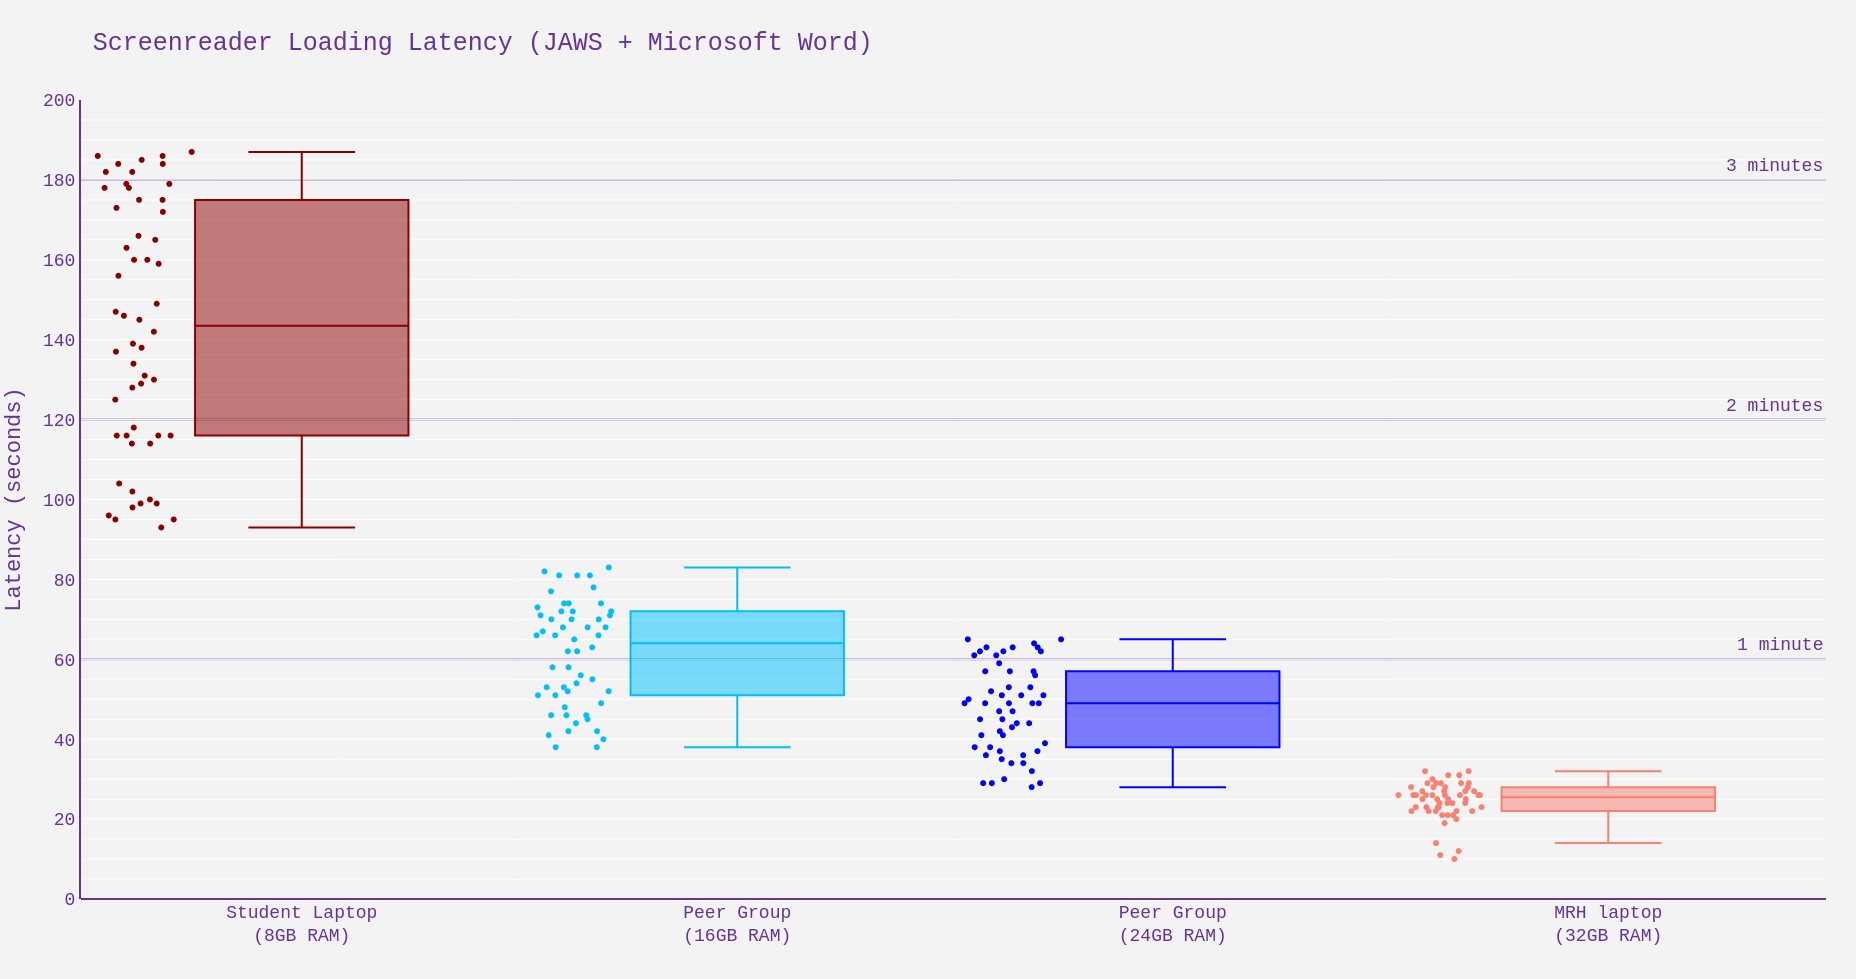
\includegraphics[width=\textwidth]{images/ComputerRBDisplaySpecsTVIFig1.png}

\caption[Latency to Load JAWS]{Plot showing Latency to Load JAWS while Microsoft Word is open across a typical student laptop (Dell Latitude 3190 with 8GB RAM), a high quality student laptop (Dell Precision 3530 with 16GB RAM), a professional laptop (Lenovo ThinkPad E16 with 24GB RAM), and a high power laptop (Microsoft Surface Laptop 3 with 32GB RAM).}\label{fig:figure 1}
\end{figure}

\pagebreak
\hypertarget{screenreader-response}{}\section{Screenreader Responsiveness}\label{screenreader-response}
Measuring the latency of a screenreader to respond to key presses is important to determine if the laptop has sufficient RAM to run the software properly. If the laptop has insufficient RAM, the screenreader may take longer to respond to key presses, which can lead to delays in the user’s workflow. Measuring the latency of a screenreader can help identify if the laptop has enough RAM to run the software smoothly. This can help users avoid frustration and improve their productivity. Additionally, measuring the latency of a screenreader can help users identify if there are other issues with their laptop that may be causing the software to run slowly. By measuring the latency of a screenreader, users can ensure that their laptop is running optimally and that they are getting the most out of their software. \textit{Table \ref{tab:table5}} provides these data for the same computers shown in Figure \ref{fig:figure 1}.

\pagebreak 
\large\textbf{\textit{Table \ref{tab:table5}}}\normalfont 
\begin{longtable}[]{
>{\raggedright\arraybackslash}m{.5\textwidth}
>{\raggedright\arraybackslash}m{.25\textwidth}
>{\raggedright\arraybackslash}b{.25\textwidth}
}
\toprule
\textbf{Computer} \break (Color as Labelled in Figure 1) & \textbf{Loading Time}\break (median [Range]) & \textbf{Response Lag}\break (median [Range]) \\
\midrule
\endhead \hline \\
\multicolumn{3}{r}{\textbf{Continued on Next Page}} \endfoot
\endlastfoot
\fcolorbox{red}{red}{\rule{0pt}{6pt}\rule{6pt}{0pt}}\qquad $\begin{array}{l}\textbf{Students Laptop}\footnote{\raggedright Dell Latitude 3190} \\ \text{8GB RAM}\end{array}$ & 143 [93-183] \footnote{\raggedright These are the data plotted in Figure 1 above. The responsiveness data are more clear when presented as a table here than as a plot} & 38 [27-91]\footnote{\raggedright It is further important to note here that any lag in screenreader responsiveness of \textgreater1 sec means the student is behind their peers and their educational opportunity is limited by the technology not being sufficient (\emph{i.e.}, not an adequate accommodation). } \\ \cdashline{1-3}
\fcolorbox{cyan}{cyan}{\rule{0pt}{6pt}\rule{6pt}{0pt}}\qquad $\begin{array}{l}\textbf{Student/Professional Laptop}\fnsep\footnote{\raggedright Dell Precision 3530} \\ \text{16GB RAM}\end{array}$ & 64 [38-93] & 9 [4-15] \\ \cdashline{1-3}
\fcolorbox{violet}{violet}{\rule{0pt}{6pt}\rule{6pt}{0pt}}\qquad$\begin{array}{l}\textbf{Professional Laptop}\footnote{\raggedright Lenovo ThinkPad E16 (TVI Personal Laptop)} \\ \text{24GB RAM}\end{array}$ & 49 [26-65] & 1 [0.05-2.5] \\ \cdashline{1-3}
\fcolorbox{orange}{orange}{\rule{0pt}{6pt}\rule{6pt}{0pt}}\qquad$\begin{array}{l}\textbf{Professional Laptop}\footnote{\raggedright Microsoft Surface 3 (My Personal Laptop)} \\ \text{32GB RAM}\end{array}$ & 25 [10-32] & 0.5 [0.01-1]\footnote{\raggedright 0.01 represents an immediate response that could not be measured} \\ [1.0em] \hline \caption{Lag in JAWS Reporting HL Content}\label{tab:table5} \\
\end{longtable}

\pagebreak \hypertarget{notes-on-future-proofing-laptops}{}\section{Laptop Cost Factors}\label{notes-on-future-proofing-laptops}
Students with visual impairments require laptops that are compatible with assistive technology to receive a free and accessible public education. When selecting a laptop, there are several cost factors that must be taken into account. Firstly, the laptop should have sufficient RAM to run the assistive technology software smoothly. Secondly, the laptop should have a high-quality screen that is large enough to display text and images clearly. Thirdly, the laptop should have a long battery life to ensure that students can use it for extended periods of time without needing to recharge. Fourthly, the laptop should have a durable build quality to withstand daily wear and tear. Finally, the laptop should be lightweight and portable to enable students to carry it around easily. These factors can help ensure that students with visual impairments have access to the technology they need to succeed in their studies.

\hypertarget{future-proofing}{}\subsection{Laptop Durability}\label{future-proofing}

I asked ChatGPT why we should consider future usage needs of a laptop into my purchasing plans and here is its response (emphasis mine):

\begin{leftbar} \begin{quote}
Buying laptops with high-end RAM and processor specifications can be beneficial for several reasons, especially in terms of longevity and performance. Here are some key considerations:

\begin{enumerate}[leftmargin=*]
\def\labelenumi{\arabic{enumi}.}

\item
Future-Proofing:
\end{enumerate}

\begin{itemize}

\item
Investing in higher-end components can help future-proof your laptop to some extent. As software and applications become more demanding over time, a laptop with better specifications is likely to remain relevant and capable of handling new software updates and requirements.
\end{itemize}

\begin{enumerate}[leftmargin=*]
\def\labelenumi{\arabic{enumi}.}
\setcounter{enumi}{1}

\item
Multitasking and Performance:
\end{enumerate}

\begin{itemize}

\item
Higher RAM allows for better multitasking capabilities. If you use resource-intensive applications or run multiple programs simultaneously, having ample RAM prevents slowdowns and ensures smooth performance.
\item
A powerful processor can handle complex computations and tasks more efficiently, contributing to faster overall system performance.
\end{itemize}

\begin{enumerate}[leftmargin=*]
\def\labelenumi{\arabic{enumi}.}
\setcounter{enumi}{2}

\item
Graphics Processing:
\end{enumerate}

\begin{itemize}

\item
For tasks such as video editing, gaming, or other graphics-intensive applications, a high-end GPU (Graphics Processing Unit) is crucial. This is separate from RAM and the main processor but is equally important for certain tasks.
\end{itemize}

\begin{enumerate}[leftmargin=*]
\def\labelenumi{\arabic{enumi}.}
\setcounter{enumi}{3}

\item
Long-Term Usability:
\end{enumerate}

\begin{itemize}

\item
Technology advances quickly, and what is considered high-end today might become standard or entry-level in a few years. However, starting with a high-end laptop gives you a more extended period before your system becomes outdated.
\end{itemize}

\begin{enumerate}[leftmargin=*]
\def\labelenumi{\arabic{enumi}.}
\setcounter{enumi}{4}

\item
Smooth Upgrades:
\end{enumerate}

\begin{itemize}

\item
Some laptops allow users to upgrade certain components like RAM and storage. Starting with higher-end specifications provides more headroom for future upgrades, allowing you to extend the useful life of your laptop.
\end{itemize}

\begin{enumerate}[leftmargin=*]
\def\labelenumi{\arabic{enumi}.}
\setcounter{enumi}{5}

\item
Resource-Intensive Applications:
\end{enumerate}

\begin{itemize}

\item
If you use applications that require a lot of processing power, like video editing software, 3D modeling tools, or virtualization software, a high-end laptop can handle these tasks more efficiently, providing a better user experience.
\end{itemize}

\begin{enumerate}[leftmargin=*]
\def\labelenumi{\arabic{enumi}.}
\setcounter{enumi}{6}

\item
Responsiveness and Speed:
\end{enumerate}

\begin{itemize}

\item
A faster processor and more RAM contribute to a more responsive system. Applications load quicker, and the overall user experience is smoother, which can significantly impact productivity.
\end{itemize}

\begin{enumerate}[leftmargin=*]
\def\labelenumi{\arabic{enumi}.}
\setcounter{enumi}{7}

\item
Enhanced Resale Value:
\end{enumerate}

\begin{itemize}

\item
High-end laptops generally retain their value better than lower-end models. If you decide to sell or upgrade your laptop in the future, having top-tier specifications can make it more attractive to potential buyers.
\end{itemize}

It's important to note that the specific requirements depend on your usage patterns and needs. Not everyone needs the highest specifications, and sometimes a mid-range laptop can be more than sufficient for everyday tasks. However, \textbf{for users with demanding workloads or those who want a longer usable life from their device, opting for higher-end specifications can be a wise investment}.
\end{quote}\end{leftbar}

\pagebreak	\hypertarget{gpu-needs}{}\subsection{Role of GPU in Laptop Performance}\label{gpu-needs}
A CPU or Central Processing Unit is the primary processor of a computer. It is responsible for executing instructions and performing calculations for all the programs running on the computer. A GPU or Graphics Processing Unit, on the other hand, is a specialized processor designed to handle complex calculations required for rendering graphics and images. While a CPU is designed to handle a wide range of tasks quickly, a GPU is designed to quickly render high-resolution images and video concurrently.

When it comes to improving laptop performance for graphics-intensive tasks or coding, a dedicated GPU can significantly improve performance. A dedicated GPU is a separate processor that is designed to handle the complex calculations required for rendering graphics and images. By offloading the processing of graphics data from the CPU, a dedicated GPU allows the CPU to focus on other tasks, resulting in faster and smoother performance for graphics-intensive applications. Additionally, a GPU can also be beneficial for processes involving AI. AI algorithms require a lot of processing power, and a GPU can help speed up the process. NVIDIA, AMD, and Intel are some of the most popular GPU manufacturers, with models available for both desktop and laptop computers. Laptops with a dedicated GPU can handle AI tasks with ease, making them ideal for professionals who work with AI.

In summary, a CPU is responsible for executing instructions and performing calculations for all the programs running on the computer, while a GPU is a specialized processor designed to handle complex calculations required for rendering graphics and images. A dedicated GPU can significantly improve laptop performance for graphics-intensive tasks such as gaming, video editing, and 3D modeling by offloading the processing of graphics data from the CPU. Screen magnification software can also benefit from a dedicated GPU. Screen magnification software enlarges the content on the screen, which can be taxing on the CPU. A dedicated GPU can help alleviate this burden by handling the graphics processing required for screen magnification. This results in a smoother and more responsive experience when using screen magnification software.

I evaluated with my personal laptop the role for a CPU and GPU in using screenreader and magnification software. I also did the same with the mid-range professional laptop with 16GB of RAM. I found there was no increase in performance for JAWS, ZDSR, NVDA, or Dolphin Screenreader when an integrated GPU was present (AMD Vega 10 or Intel UHD Graphics 630 integrated GPU). However, when I assessed performance of ZoomText, Fusion (ZoomText + JAWS), and Dolphin SuperNova magnifier, as well as Dolphin Magnifier + ScreenReader, I saw a 30-45\% increase in responsiveness for both speech and visual markers available on the screen. In this case I opened 10 tabs in Google Chrome, 10 tabs in Microsoft Edge, 10 tabs in Mozilla Firefox, and started typing in an online Microsoft Word document using office 365 online. Response time refers to the time it took the system to react when I typed beyond the field of view and the system had to move the screen and visual screen marker to a new location. Table \ref{tab:table51} shows these data. Importantly, both of the laptops were able to improve their performance for Magnification tasks by a similar percentage when the integrated GPU was used in concert with the CPU.

\pagebreak 
\large\textbf{Table \ref{tab:table51}}\normalfont 
\begin{longtable}[]{
>{\raggedright\arraybackslash}m{.3\textwidth}
>{\raggedright\arraybackslash}m{.25\textwidth}
>{\raggedright\arraybackslash}m{.25\textwidth}
>{\raggedright\arraybackslash}m{.2\textwidth}
}
\toprule & \textbf{CPU} & \textbf{CPU + GPU} & \textbf{\% Improvement} \\
\midrule
\endhead \hline \\
\multicolumn{2}{r}{\textbf{Continued on Next Page}} \endfoot
\endlastfoot
\multicolumn{2}{l}{\textbf{Screenreader Only}\footnote{\raggedright The visual marker outlining the current focus was used to measure response}} \\
JAWS Screenreader & $\begin{array}{l}0.5~~[0.01-1] \\9.0~~[4-15]\end{array}$ & $\begin{array}{l}0.5~~[0.01-1] \\9.0~~[3-17]\end{array}$ & $\begin{array}{l} 0\% \\ 0\%\end{array}$ \\ \cdashline{2-4}
JAWS Screenreader & $\begin{array}{l}0.5~~[0.01-1] \\9.0~~[4-15]\end{array}$ & $\begin{array}{l}0.5~~[0.01-1] \\9.0~~[3-17]\end{array}$ & $\begin{array}{l} 0\% \\ 0\%\end{array}$ \\ \cdashline{2-4}
NVDA Screenreader & $\begin{array}{l}0.2~~[0.01-0.5] \\4.0~~[1.5-6]\end{array}$ & $\begin{array}{l}0.2~~[0.01-0.5] \\4.0~~[1.5-6]\end{array}$ & $\begin{array}{l} 0\% \\ 0\%\end{array}$ \\ \cdashline{2-4}
Dolphin Screenreader & $\begin{array}{l}0.5~~[0.01-1] \\9.0~~[5-17]\end{array}$ & $\begin{array}{l}0.5~~[0.01-1] \\8.8~~[5-17]\end{array}$ & $\begin{array}{l} 0\% \\ 2\%\end{array}$ \\ \cdashline{2-4}
ZDSR Screenreader & $\begin{array}{l}0.2~~[0.01-0.75] \\5.0~~[2-7]\end{array}$ & $\begin{array}{l}0.2~~[0.01-0.75] \\5.0~~[2-7]\end{array}$ & $\begin{array}{l} 0\% \\ 0\%\end{array}$ \\ \cdashline{2-4}
\multicolumn{2}{l}{\textbf{Screen Magnification Only}\footnotemark[48]} \\
ZoomText & $\begin{array}{l}1.1~~[0.5-1.25] ] \\15~~~[10-19]\end{array}$ & $\begin{array}{l}.75~~[0.3-1] ] \\5~~~~~[2.5-10]\end{array}$ & $\begin{array}{l} 32\% \\ 33\%\end{array}$ \\ \cdashline{2-4}
SuperNova & $\begin{array}{l}1.5~~[0.75-1.45] \\11~~~[4-20]\end{array}$ & $\begin{array}{l}.77~~[0.4-1] \\7~~~~~[3-11]\end{array}$ & $\begin{array}{l} 48\% \\ 36\%\end{array}$ \\ \cdashline{2-4}
\multicolumn{2}{l}{\textbf{Screenreader + Magnification}\footnotemark[48]} \\
SuperNova + Magnification & $\begin{array}{l}1.5~~[1-25] ] \\16~~~[9-25]\end{array}$ & $\begin{array}{l}.75~~[0.25-1] ] \\6~~~~~[3-15]\end{array}$ & $\begin{array}{l} 48\% \\ 37\%\end{array}$ \\ \cdashline{2-4}
Fusion & $\begin{array}{l}1.5~~[1-1.75] \\13~~~[3-19]\end{array}$ & $\begin{array}{l}.75~~[0.25-1] \\5~~~~~[2.5-13]\end{array}$ & $\begin{array}{l} 48\% \\ 38\%\end{array}$ \\[1.0em]\hline
\caption[Screen Magnifiers Benefit from Integrated GPU]{Screen Magnifiers Benefit from Use of an Integrated GPU. The top row in each table cell contains data for the laptop with 32GB RAM, an AMD Ryzen 7 processor and AMD Vega 10 integrated GPU. The lower crow in each cell contains data for the laptop with 16GB RAM, an 8th Gen 17 processor, and Intel UHD 630 integrated GPU.} \label{tab:table51}
\end{longtable}

\pagebreak	\hypertarget{optimizing-cost-with-performance}{}\subsection{Laptop Cost Optimization}\label{optimizing-cost-with-performance}

There is an economic theory based on a Terry Pratchett novel that explains this phenomenon better than we can. It is called the \href{http://en.wikipedia.org/wiki/Boots_theory}{Boots Theory}\footnote{\raggedright Full Text (emphasis mine):
\begin{leftbar}
\begin{quote}The reason that the rich were so rich, Vimes reasoned, was because they managed to spend less money.

Take boots, for example. He earned thirty-eight dollars a month plus allowances. A really good pair of leather boots cost fifty dollars. But an affordable pair of boots, which were sort of OK for a season or two and then leaked like hell when the cardboard gave out, cost about ten dollars. Those were the kind of boots Vimes always bought, and wore until the soles were so thin that he could tell where he was in Ankh-Morpork on a foggy night by the feel of the cobbles.

But the thing was that good boots lasted for years and years. \textbf{A man who could afford fifty dollars had a pair of boots that’d still be keeping his feet dry in ten years’ time, while the poor man who could only afford cheap boots would have spent a hundred dollars on boots in the same time and would still have wet feet.}

Basically, \textbf{we are destined to be stuck in a cycle of perpetually spending more money for inferior products and will, in the end, spend more money than if we just paid for better product in the first place.} \break \qquad-- \textit{Men At Arms}, page 38
\end{quote}
\end{leftbar} 
}

\hfill \break \textit{Table \ref{tab:table6}} illustrates this theory in terms of student laptop computers (Assuming student has a laptop using a screenreader through 3rd-12th grade). \textit{Table \ref{tab:table6}} also illustrates why we choose to err on the side of spending \$2000-3000 on a laptop computer that will last 3-5 years over spending \$1500-2000 on a laptop that will reach end-of-life within 1-2 years before becoming obsolete. By the end of 5 years we will have spent more on Low End and Mid Range Laptops than we would have otherwise spent had we purchased a High End Laptop. Importantly; however, we also would have been using laptops that always performed more poorly than a High End laptop would.

\pagebreak 
\large\textbf{\textit{Table \ref{tab:table6}}}\normalfont 
\begin{longtable}[]{
>{\raggedright\arraybackslash}m{.15\textwidth}
>{\raggedright\arraybackslash}m{.05\textwidth}
>{\raggedright\arraybackslash}m{.05\textwidth}
>{\raggedright\arraybackslash}m{.05\textwidth}
>{\raggedright\arraybackslash}m{.05\textwidth}
>{\raggedright\arraybackslash}m{.05\textwidth}
>{\raggedright\arraybackslash}m{.05\textwidth}
>{\raggedright\arraybackslash}m{.05\textwidth}
>{\raggedright\arraybackslash}m{.05\textwidth}
>{\raggedright\arraybackslash}m{.05\textwidth}
>{\raggedright\arraybackslash}m{.05\textwidth}
>{\raggedright\arraybackslash}b{.10\textwidth}
}
\toprule & \multicolumn{10}{c}{\textbf{Does School Have to Purchase a Replacement Laptop by Year}} & \\ \cdashline{1-12}
\cline{2-11} \\
\textbf{RAM} \break Cost & \textbf{1} & \textbf{2} & \textbf{3} & \textbf{4} & \textbf{5} & \textbf{6} & \textbf{7} & \textbf{8} & \textbf{9} & \textbf{10} & \textbf{10-year Cost} \\
\midrule
\endhead \hline \\
\multicolumn{6}{r}{\textbf{Continued on Next Page}} \endfoot
\endlastfoot
\textbf{4GB}\footnote{\raggedright Dell Latitude 3190 Education}\fnsep\footnote{\raggedright The 4GB Laptop \textit{cannot} run JAWS and is included to show price comparison to the other options} \break \$525.04 & $\checkmark$ & $\checkmark$ & $\checkmark$ & $\checkmark$ & $\checkmark$ & $\checkmark$ & $\checkmark$ & $\checkmark$ & $\checkmark$ & $\checkmark$ & \$5,250 \\ \cdashline{1-12}
\textbf{8GB}\footnote{\raggedright Dell Latitude 3190 Education}  \break \$1184 & $\checkmark$ & $\checkmark$ & $\checkmark$ & $\checkmark$ & $\checkmark$ & $\checkmark$ & $\checkmark$ & $\checkmark$ & $\checkmark$ & $\checkmark$ & \$11,840 \\ \cdashline{1-12}
\textbf{16GB}\footnote{\raggedright Dell Precision 3530 given to TVIs teaching screenreaders} \break \$1751 & $\checkmark$ & - & $\checkmark$ & - & $\checkmark$ & - & $\checkmark$ & - & $\checkmark$ & - & \$8,755 \\ \cdashline{1-12}
\cdashline{1-12} \\
\textbf{32GB}\footnote{\raggedright Microsoft Surface Laptop 3}\break \$2824\break \textcolor{red}{\textit{Best Case}}\footnote{\raggedright This is my personal experience} & $\checkmark$ & - & - & - & - & $\checkmark$ & - & - & - & - & \$5,648 \\ \cdashline{1-12}
\textbf{32GB}\footnote{\raggedright Microsoft Surface Laptop 3}\break \$2824\break \textcolor{red}{\textit{Cautious}}\footnote{\raggedright This is a conservative estimate to account for potential rough treatment of a computer} & $\checkmark$ & - & - & $\checkmark$ & - & - & $\checkmark$ & - & - & - & \$8,472 \\[1.0em]\hline
\caption[Cost of Laptops over Time]{Cost of Laptops Across Time. Notice that the final cost of the 32GB option is comparable to the 4GB over 10 years. However, the 4GB laptop is not capable of running JAWS reliably in the classroom setting.
\break\textbullet For the \textcolor{red}{Best Case} Scenario, the 32GB laptop is between \$3,107 and \$6,192 \textit{\textbf{cheaper}} over time compared to the 16GB and 8GB laptops, respectively.
\break\textbullet For the \textcolor{red}{Cautious} Scenario, the 32GB laptop is between \$283 and \$3,386 \textit{\textbf{cheaper}} over time compared to the 16GB and 8GB laptops, respectively}\label{tab:table6}
\end{longtable}

\pagebreak
\hypertarget{minimum-laptop-recommendations}{}\section{Recommended Laptop Specifications}\label{minimum-laptop-recommendations}
\textit{Table \ref{tab:table7}} is a list of recommendations for laptop specifications by use case.

\pagebreak 
\large\textbf{\textit{Table \ref{tab:table7}}}\normalfont 
\begin{longtable}[]{
>{\raggedright\arraybackslash}m{.7\textwidth}
>{\raggedright\arraybackslash}b{.3\textwidth}
}
\toprule

\textbf{Use Case} & \textbf{Recommendation} \\
\midrule
\endhead \hline \\
\multicolumn{2}{r}{\textbf{Continued on Next Page}} \endfoot
\endlastfoot
\multicolumn{2}{l}{\textbf{Screenreader Only}} \\[1em]
JAWS Screenreader \\ \cdashline{1-2}
NVDA Screenreader & \textgreater24-32GB \\ \cdashline{1-2}
Dolphin Screenreader & \textgreater24-32GB \\ \cdashline{1-2}
ZDSR Screenreader & \textgreater24-32GB \\ \cdashline{1-2}
\multicolumn{2}{l}{\textbf{Screen Magnification Only}\footnote{can also benefit from either an integrated or dedicated GPU}} \\[1em]
ZoomText & \textgreater24-32GB \\ \cdashline{1-2}
Windows Magnifier & \textgreater16GB \\ \cdashline{1-2}
Dolphin SuperNova & \textgreater24-32GB \\ \cdashline{1-2}
\multicolumn{2}{l}{\textbf{Screenreader + Magnification}\footnotemark[\value{footnote}]} \\[1em]
JAWS Screenreader + Windows Magnifier & \textgreater24-32GB \\ \cdashline{1-2}
NVDA Screenreader + Windows Magnifier & \textgreater24-32GB \\ \cdashline{1-2}
ZDSR Screenreader + Windows Magnifier & \textgreater24-32GB \\ \cdashline{1-2}
Dolphin Screenreader + Windows Magnifier & \textgreater24-32GB \\ \cdashline{1-2}
SuperNova Screenreader + Magnification & \textgreater32-64GB \\ \cdashline{1-2}
Fusion Screenreader + Magnification & \textgreater32-64GB \\\hline
\caption{Recommended Laptop Specifications}\label{tab:table7}
\end{longtable}

\pagebreak
\hypertarget{laptops-meeting-recommended-specifications}{}\section{Laptops Meeting Specifications}\label{laptops-meeting-recommended-specifications}
\textit{Table \ref{tab:table8}} is an alphabetical list of laptop computers that meet the recommended specifications defined in \textit{Table \ref{tab:table7}}.

\pagebreak 
\large\textbf{\textit{Table \ref{tab:table8}}}\normalfont 
\begin{longtable}[]{
>{\raggedright\arraybackslash}m{.3\textwidth}
>{\raggedright\arraybackslash}m{.12\textwidth}
>{\raggedright\arraybackslash}m{.12\textwidth}
>{\raggedright\arraybackslash}m{.12\textwidth}
>{\raggedright\arraybackslash}b{.2\textwidth}
}
\toprule
\textbf{Company / Model} & \textbf{Cost} & \textbf{RAM} & \textbf{Display} & \textbf{Processor} \\
\midrule
\endhead \hline \\
\multicolumn{5}{r}{\textbf{Continued on Next Page}} \endfoot
\endlastfoot
\multicolumn{5}{l}{\textbf{Screenreader Only\footnote{\raggedright Laptops without integrated/dedicated GPU units}}} \\ \cdashline{1-5}
\multicolumn{5}{l}{\break\textbf{\qquad\$1000-\$2000}} \\ \cdashline{1-5}
Acer Aspire 5 & \$1319 & 32GB & 15.6 & 13th Gen i7 \\ \cdashline{1-5}
ASUS Vivobook 17X & \$1149 & 32GB & 17.3 & AMD Ryzen 7 \\ \cdashline{1-5}
ASUS Vivobook 17X & \$1189 & 40GB & 17.3 & AMD Ryzen 7 \\ \cdashline{1-5}
ASUS Vivobook 17X & \$1249 & 40GB & 17.3 & 13th Gen i9 \\ \cdashline{1-5}
BT Speak Pro\footnote{\raggedright This is a Linux computer with Perkins-style input and auditory output} & \$1,195 & TBD & none & TBD \\ \cdashline{1-5}
Dell G16 Gaming Laptop & \$1,999 & 32GB & 16.0 & 13th Gen i7 \\ \cdashline{1-5}
Dell Inspiron 16 Plus & \$1,499 & 32GB & 16.0 & 13th Gen i7 \\ \cdashline{1-5}
Dell Inspiron 3530 & \$1259 & 32GB & 15.6 & 13th Gen i7 \\ \cdashline{1-5}
Dell Inspiron 3530 & \$1339 & 48GB & 15.6 & 13th Gen i7 \\ \cdashline{1-5}
Dell Inspiron 3530 & \$1419 & 64GB & 15.6 & 13th Gen i7 \\ \cdashline{1-5}
Dell XPS 9530 & \$1829 & 32GB & 15.6 & 13th Gen i7 \\ \cdashline{1-5}
Dell XPS 9530 & \$1929 & 48GB & 15.6 & 13th Gen i7 \\ \cdashline{1-5}
Framework 13 & \$1,102 & 32GB & 13.5 & 13th Gen i7 \\ \cdashline{1-5}
Framework 13 & \$1,732 & 32GB & 13.5 & AMD Ryzen 7 \\ \cdashline{1-5}
Framework 13 & \$1,892 & 64GB & 13.5 & AMD Ryzen 7 \\ \cdashline{1-5}
HP 14 & \$1189 & 32GB & 14.0 & 13th Gen i7 \\ \cdashline{1-5}
HP 14 & \$1269 & 48GB & 14.0 & 13th Gen i7 \\ \cdashline{1-5}
HP 14 & \$1349 & 64GB & 14.0 & 13th Gen i7 \\ \cdashline{1-5}
HP 15 & \$1879 & 64GB & 15.6 & 13th Gen i7 \\ \cdashline{1-5}
HP 17 & \$1019 & 32GB & 17.3 & AMD Ryzen 7 \\ \cdashline{1-5}
HP 17 & \$1449 & 64GB & 17.3 & 13th Gen i7 \\ \cdashline{1-5}
HP 17 & \$1802 & 64GB & 17.3 & 13th Gen i7 \\ \cdashline{1-5}
HP 17 & \$1929 & 64GB & 17.3 & AMD Ryzen 7 \\ \cdashline{1-5}
HP Dragonfly Pro & \$1,549 & 32GB & 14.0 & AMD Ryzen 7 \\ \cdashline{1-5}
HP EliteBook 860 G10 & \$1819 & 64GB & 16.0 & 13th Gen i7 \\ \cdashline{1-5}
HP Envy & \$1,749 & 32GB & 17.3 & 13th Gen i7 \\ \cdashline{1-5}
HP ENVY x360 15 & \$1059 & 64GB & 15.6 & AMD Ryzen 7 \\ \cdashline{1-5}
HP ENVY x360 15 & \$1519 & 32GB & 15.6 & 13th Gen i7 \\ \cdashline{1-5}
HP ENVY x360 15 & \$1599 & 48GB & 15.6 & 13th Gen i7 \\ \cdashline{1-5}
HP ENVY x360 15 & \$1679 & 64GB & 15.6 & 13th Gen i7 \\ \cdashline{1-5}
HP Pavilion 15 & \$1329 & 48GB & 15.6 & AMD Ryzen 7 \\ \cdashline{1-5}
HP Pavilion 15 & \$1359 & 32GB & 15.6 & 13th Gen i7 \\ \cdashline{1-5}
HP Pavilion 15 & \$1409 & 64GB & 15.6 & AMD Ryzen 7 \\ \cdashline{1-5}
HP Pavilion 15 & \$1439 & 48GB & 15.6 & 13th Gen i7 \\ \cdashline{1-5}
HP ZBook Firefly 16 G10 & \$1934 & 32GB & 16.0 & 13th Gen i7 \\ \cdashline{1-5}
Lenovo ThinkPad E16 Gen 1 & \$1309 & 32GB & 16.0 & AMD Ryzen 7 \\ \cdashline{1-5}
Lenovo ThinkPad E16 Gen 1 & \$1349 & 40GB & 16.0 & AMD Ryzen 7 \\ \cdashline{1-5}
Lenovo ThinkPad E16 Gen 1 & \$1459 & 32GB & 16.0 & 13th Gen i7 \\ \cdashline{1-5}
Lenovo ThinkPad E16 Gen 1 & \$1599 & 40GB & 16.0 & 13th Gen i7 \\ \cdashline{1-5}
Lenovo ThinkPad T16 Gen 2 & \$1994 & 32GB & 16.0 & 13th Gen i7 \\ \cdashline{1-5}
Lenovo Yoga 7i 14 & \$1399 & 32GB & 14.0 & 13th Gen i7 \\ \cdashline{1-5}
LG Gram 14 & \$1,699 & 32GB & 14.4 & 13th Gen i7 \\ \cdashline{1-5}
LG Gram 14 & \$1,799 & 64GB & 14.4 & 13th Gen i7 \\ \cdashline{1-5}
LG Gram 16 & \$1,999 & 32GB & 16.0 & 13th Gen i7 \\ \cdashline{1-5}
LG gram 17 & \$1769 & 32GB & 17.0 & 13th Gen i7 \\ \cdashline{1-5}
Malibal Aon L1 & \$1,589 & 32GB & 16.0 & 13th Gen i7 \\ \cdashline{1-5}
Malibal Aon L1 & \$1,625 & 64GB & 16.0 & 13th Gen i7 \\ \cdashline{1-5}
MSI Commercial 14 & \$1279 & 32GB & 14.0 & 13th Gen i7 \\ \cdashline{1-5}
MSI Commercial 14 & \$1579 & 64GB & 14.0 & 13th Gen i7 \\ \cdashline{1-5}
MSI Prestige 14 & \$1529 & 32GB & 14.0 & 13th Gen i7 \\ \cdashline{1-5}
MSI Prestige 16 & \$1699 & 32GB & 16.0 & 13th Gen i7 \\ \cdashline{1-5}
MSI Summit E14 Flip & \$1829 & 32GB & 14.0 & 13th Gen i7 \\ \cdashline{1-5}
Overpowered 17+ & \$1,699 & 32GB & 17.3 & 13th Gen i7 \\ \cdashline{1-5}
\multicolumn{5}{l}{\break\textbf{\qquad\$2000-\$3000}} \\ \cdashline{1-5}
ASUS ProArt Studiobook & \$2,999 & 32GB & 16.0 & 13th Gen i9 \\ \cdashline{1-5}
ASUS Zenbook Pro 16X & \$2,599 & 32GB & 16.0 & 13th Gen i9 \\ \cdashline{1-5}
Dell XPS 13 Plus & \$2,009 & 32GB & 13.4 & 13th Gen i7 \\ \cdashline{1-5}
Dell XPS 15 & \$2,999 & 32GB & 15.6 & 13th Gen i9 \\ \cdashline{1-5}
Dell XPS 9530 & \$2029 & 64GB & 15.6 & 13th Gen i7 \\ \cdashline{1-5}
Framework 13 & \$2,222 & 64GB & 13.5 & 13th Gen i7 \\ \cdashline{1-5}
Framework 16 & \$2,239\footnote{with NUMPAD} & 32GB & 16.0 & AMD Ryzen 9 \\ \cdashline{1-5}
Framework 16 & \$2,399\footnotemark[60] & 64GB & 16.0 & AMD Ryzen 9 \\ \cdashline{1-5}
HP ZBook Firefly 16 G10 & \$2549 & 64GB & 16.0 & 13th Gen i7 \\ \cdashline{1-5}
Legion Pro 7i & \$3,599 & 32GB & 16.0 & 13th Gen i9 \\ \cdashline{1-5}
Lenovo Thinkpad P14s & \$2,199 & 32GB & 14.0 & AND Ryzen 7 \\ \cdashline{1-5}
Lenovo Thinkpad P14s & \$2,509 & 64GB & 14.0 & AND Ryzen 7 \\ \cdashline{1-5}
Lenovo ThinkPad P16 Gen 2 & \$2,039 & 32GB & 16.0 & AMD Ryzen 7 \\ \cdashline{1-5}
Lenovo ThinkPad P16 Gen 2 & \$2,829 & 64GB & 16.0 & AMD Ryzen 7 \\ \cdashline{1-5}
Lenovo ThinkPad T16 Gen 2 & \$2254 & 48GB & 16.0 & 13th Gen i7 \\ \cdashline{1-5}
LG gram 16 2-in-1 & \$2119 & 32GB & 16.0 & 13th Gen i7 \\ \cdashline{1-5}
LG Gram 17 & \$2,099 & 32GB & 17.3 & 13th Gen i7 \\ \cdashline{1-5}                           
\multicolumn{5}{l}{\break\textbf{\qquad\$3000-\$4000}} \\ \cdashline{1-5}
Dell Latitude 7440 & \$3,615 & 32GB & 14.0 & 13th Gen i7 \\ \cdashline{1-5}
Dell Precision 3480 & \$3,205 & 32GB & 14.0 & 13th Gen i7 \\ \cdashline{1-5}
Dell Precision 3581 & \$3,854 & 32GB & 15.6 & 13th Gen i7 \\ \cdashline{1-5}
Dell XPS 17 & \$3,349 & 32GB & 15.6 & 13th Gen i7 \\ \cdashline{1-5}
Dell XPS 17 & \$3,549 & 32GB & 15.6 & 13th Gen i9 \\ \cdashline{1-5}
Lenovo ThinkPad P16 Gen 2 & \$3,239 & 32GB & 16.0 & 13th Gen i7 \\ \cdashline{1-5}
Lenovo ThinkPad P16v & \$3,339 & 32GB & 16.0 & 13th Gen i7 \\ \cdashline{1-5}
Lenovo Thinkpad X1 Yoga & \$3,719 & 32GB & 14.0 & 13th Gen i7 \\ \cdashline{1-5}
\multicolumn{5}{l}{\break\textbf{\qquad\textgreater\$4000}} \\ \cdashline{1-5}
b.book\footnote{\raggedright This is a Windows Computer without a monitor, substituting a 40 cell braille display} & \$5,765 & 8GB-16GB & none & 13th Gen i9 \\ \cdashline{1-5}
Dell Precision 5480 & \$4,354 & 32GB & 14.0 & 13th Gen i7 \\ \cdashline{1-5}
Dell Precision 5680 & \$5,597 & 32GB & 16.0 & 13th Gen i9 \\ \cdashline{1-5}
Dell Precision 7680 & \$7,225 & 32GB & 16.0 & 13th Gen i9 \\ \cdashline{1-5}
Lenovo ThinkPad P16 Gen 2 & \$4,189 & 64GB & 16.0 & 13th Gen i7 \\ \cdashline{1-5}
Lenovo ThinkPad P16v & \$4,929 & 64GB & 16.0 & 13th Gen i7 \\ \cdashline{1-5}
Orbit Optima\footnotemark[\value{footnote}] & \$6,500 & 32GB-64GB & none & 13th Gen i7 \\ \cdashline{1-5}
Seika Studio\footnotemark[\value{footnote}] & \$6,500 & 8GB-16GB\footnotemark[62] & none & 12th Gen i7 \\ \cdashline{1-5}
\multicolumn{5}{l}{\textbf{Screenreader OR Magnification + Screenreader}} \\
\multicolumn{5}{l}{\break\textbf{\qquad\$1000-\$2000}} \\
Alienware x14\footnote{\raggedright with NVIDIA GeForce RTX 4080} & \$1,999 & 32GB & 14.0 & 13th Gen i7 \\ \cdashline{1-5}
ASUS ROG Zephyrus G14\footnotemark[65] & \$1819 & 32GB & 14.0 & AMD Ryzen 7 \\ \cdashline{1-5}
ASUS ROG Zephyrus G14\footnotemark[65] & \$1889 & 48GB & 14.0 & AMD Ryzen 7 \\ \cdashline{1-5}
ASUS ROG Zephyrus G14\footnotemark[65] & \$1699 & 40GB & 14.0 & AMD Ryzen 9 \\ \cdashline{1-5}
ASUS ROG Zephyrus G16\footnotemark[65] & \$1989 & 32GB & 16.0 & 13th Gen i7 \\ \cdashline{1-5}
ASUS TUF Gaming A15\footnotemark[65] & \$1549 & 32GB & 15.6 & AMD Ryzen 7 \\ \cdashline{1-5}
ASUS TUF Gaming A16\footnote{\raggedright  AMD Radeon RX 7600S} & \$1445 & 32GB & 16.0 & AMD Ryzen 7 \\ \cdashline{1-5}
ASUS Vivobook 16X\footnote{\raggedright  with NVIDIA GeForce RTX 3050} & \$1739 & 40GB & 16.0 & 13th Gen i9 \\ \cdashline{1-5}
ASUS Vivobook 16X\footnotemark[65] & \$1829 & 32GB & 16.0 & 13th Gen i9 \\ \cdashline{1-5}
ASUS Vivobook 16X\footnotemark[65] & \$1909 & 48GB & 16.0 & 13th Gen i9 \\ \cdashline{1-5}
Eluktronics RP-15 G2\footnote{\raggedright with NVIDIA GeForce RTX 4060} & \$1,797 & 64GB & 15.6 & AMD Ryzen 7 \\ \cdashline{1-5}
HP Pavilion 15\footnote{\raggedright  with NVIDIA GeForce e MX550} & \$1309 & 32GB & 15.6 & 13th Gen i7 \\ \cdashline{1-5}
HP Pavilion 15\footnotemark[65] & \$1389 & 48GB & 15.6 & 13th Gen i7 \\ \cdashline{1-5}
HP Pavilion 15\footnotemark[65] & \$1469 & 64GB & 15.6 & 13th Gen i7 \\ \cdashline{1-5}
HP Victus 16\footnotemark[65] & \$1599 & 32GB & 16.1 & AMD Ryzen 7 \\ \cdashline{1-5}
HP Victus 16\footnotemark[65] & \$1699 & 64GB & 16.1 & AMD Ryzen 7 \\ \cdashline{1-5}
Lenovo IdeaPad Gaming 3 15\footnotemark[65] & \$1079 & 64GB & 15.6 & AMD Ryzen 7 \\ \cdashline{1-5}
Lenovo IdeaPad Gaming 3 15\footnotemark[65] & \$1149 & 32GB & 15.6 & AMD Ryzen 7 \\ \cdashline{1-5}
Malibal Aon L1\footnotemark[65] & \$1,589 & 32GB & 16.0 & 13th Gen i7 \\ \cdashline{1-5}
Malibal Aon S1\footnotemark[67] & \$1,812 & 32GB & 14.0 & 13th Gen i7 \\ \cdashline{1-5}
MSI Alpha 17\footnote{\raggedright with AMD Radeon RX5500M} & \$1,849 & 32GB & 17.3 & AMD Ryzen9 \\ \cdashline{1-5}
MSI Bravo 15\footnotemark[65] & \$1189 & 32GB & 15.6 & AMD Ryzen 7 \\ \cdashline{1-5}
MSI Bravo 15\footnotemark[65] & \$1279 & 64GB & 15.6 & AMD Ryzen 7 \\ \cdashline{1-5}
MSI Bravo 17\footnotemark[68] & \$1,499 & 32GB & 17.3 & AMD Ryzen7 \\ \cdashline{1-5}
MSI Crosshair 16\footnotemark[65] & \$1699 & 32GB & 16.0 & 13th Gen i7 \\ \cdashline{1-5}
MSI Crosshair 16\footnotemark[65] & \$1809 & 64GB & 16.0 & 13th Gen i7 \\ \cdashline{1-5}
MSI Cyborg 15\footnotemark[65] & \$1699 & 48GB & 15.6 & 13th Gen i7 \\ \cdashline{1-5}
MSI Cyborg 15\footnotemark[65] & \$1874 & 32GB & 15.6 & 13th Gen i7 \\ \cdashline{1-5}
MSI Cyborg\footnotemark[65] & \$1,240 & 32GB & 15.6 & AMD Ryzen7 \\ \cdashline{1-5}
MSI Katana 15\footnotemark[65] & \$1,899 & 32GB & 15.6 & 13th Gen i9 \\ \cdashline{1-5}
MSI Pulse 17\footnotemark[70] & \$1,899 & 32GB & 17.3 & 13th Gen i9 \\ \cdashline{1-5}
MSI Pulse 15\footnotemark[65] & \$1599 & 32GB & 15.6 & 13th Gen i7 \\ \cdashline{1-5}
MSI Pulse 15\footnote{\raggedright with NVIDIA GeForce RTX 3060} & \$1,699 & 32GB & 15.6 & 13th Gen i7 \\ \cdashline{1-5}
MSI Raider 15\footnote{\raggedright with NVIDIA GeForce RTX 3070} & \$1,999 & 32GB & 15.6 & 13th Gen i9 \\ \cdashline{1-5}
MSI Stealth 14 Studio\footnotemark[65] & \$1949 & 64GB & 14.0 & 13th Gen i7 \\ \cdashline{1-5}
MSI Vector\footnotemark[71] & \$1,999 & 32GB & 17.3 & 13th Gen i9 \\ \cdashline{1-5}
Sager NP8855D\footnotemark[65] & \$1,549 & 32GB & 15.6 & 13th Gen i9 \\ \cdashline{1-5}
Sager NP8855D\footnotemark[65] & \$1,704 & 64GB & 15.6 & 13th Gen i9 \\ \cdashline{1-5}
Sager NP8875E\footnotemark[66] & \$1,799 & 32GB & 17.3 & 13th Gen i9 \\ \cdashline{1-5}
Sager NP8875E\footnotemark[66] & \$1,954 & 64GB & 17.3 & 13th Gen i9 \\ \cdashline{1-5}
XPG Xenia 15G\footnotemark[66] & \$1,399 & 32GB & 15.6 & 13th Gen i7 \\ \cdashline{1-5}
\multicolumn{5}{l}{\break\textbf{\qquad\$2000-\$4000}} \\ \cdashline{1-5}
Acer Predator Helios 16\footnotemark[65] & \$2,499 & 32GB & 16.0 & 13th Gen i9 \\ \cdashline{1-5}
Acer Predator Triton\footnotemark[65] & \$3,799 & 64GB & 17.0 & 13th Gen i9 \\ \cdashline{1-5}
Alienware m16\footnotemark[65] & \$3,499 & 32GB & 16.0 & 13th Gen 19 \\ \cdashline{1-5}
ASUS Creator Laptop Q\footnotemark[67] & \$2799 & 40GB & 15.6 & 13th Gen i9 \\ \cdashline{1-5}
ASUS ROG Flow X16\footnotemark[65] & \$2489 & 32GB & 16.0 & 13th Gen i9 \\ \cdashline{1-5}
ASUS ROG Flow X16\footnotemark[65] & \$3059 & 64GB & 16.0 & 13th Gen i9 \\ \cdashline{1-5}
ASUS ROG Zephyrus G14\footnotemark[65] & \$2359 & 48GB & 14.0 & AMD Ryzen 9 \\ \cdashline{1-5}
ASUS ROG Zephyrus G14\footnotemark[65] & \$2419 & 32GB & 14.0 & AMD Ryzen 9 \\ \cdashline{1-5}
ASUS ROG Zephyrus G16\footnotemark[65] & \$2039 & 48GB & 16.0 & 13th Gen i7 \\ \cdashline{1-5}
ASUS ROG Zephyrus M16\footnotemark[65] & \$2079 & 32GB & 16.0 & 13th Gen i9 \\ \cdashline{1-5}
ASUS ROG Zephyrus M16\footnotemark[65] & \$2369 & 64GB & 16.0 & 13th Gen i9 \\ \cdashline{1-5}
ASUS ROG Zephyrus M16\footnotemark[64] & \$3289 & 96GB & 16.0 & 13th Gen i9 \\ \cdashline{1-5}
ASUS TUF Gaming A15\footnotemark[65] & \$2069 & 64GB & 15.6 & AMD Ryzen 9 \\ \cdashline{1-5}
ASUS TUF Gaming A16\footnote{\raggedright with AMD Radeon RX 7700S} & \$2119 & 64GB & 16.0 & AMD Ryzen 9 \\ \cdashline{1-5}
ASUS Vivobook Pro 16X\footnotemark[65] & \$2339 & 32GB & 16.0 & 13th Gen i9 \\ \cdashline{1-5}
ASUS Vivobook Pro 16X\footnotemark[65] & \$2349 & 64GB & 16.0 & 13th Gen i9 \\ \cdashline{1-5}
ASUS Zenbook Pro 14\footnotemark[65] & \$2779 & 48GB & 14.5 & 13th Gen i9 \\ \cdashline{1-5}
ASUS Zenbook Pro 14\footnotemark[65] & \$2199 & 32GB & 14.5 & 13th Gen i9 \\ \cdashline{1-5}
Corsair Voyager\footnote{\raggedright with AMD Radeon 6800M} & \$2,350 & 32GB & 16.0 & AMD Ryzen 9 \\ \cdashline{1-5}
Dell XPS 9530\footnotemark[65] & \$2399 & 32GB & 15.6 & 13th Gen i7 \\ \cdashline{1-5}
Dell XPS 9530\footnotemark[65] & \$2599 & 64GB & 15.6 & 13th Gen i7 \\ \cdashline{1-5}
Dell XPS 9730\footnotemark[64] & \$3899 & 32GB & 17.0 & 13th Gen i9 \\ \cdashline{1-5}
Dell XPS 9730\footnotemark[64] & \$5299 & 64GB & 17.0 & 13th Gen i9 \\ \cdashline{1-5}
DigitalStorm Nova\footnotemark[66] & \$2,294 & 32GB & 16.0 & 13th Gen i9 \\ \cdashline{1-5}
DigitalStorm Nova\footnotemark[66] & \$2,428 & 64GB & 16.0 & 13th Gen i9 \\ \cdashline{1-5}
Falcon NW TLX\footnotemark[65] & \$2,423 & 32GB & 16.0 & 13th Gen i9 \\ \cdashline{1-5}
Falcon NW TLX\footnotemark[65] & \$2,567 & 64GB & 16.0 & 13th Gen i9 \\ \cdashline{1-5}
Framework 16\footnotemark[73] & \$2,808& 64GB & 16.0 & AMD Ryzen 9 \\ \cdashline{1-5}
Framework 16\footnotemark[74] & \$2,639& 32GB & 16.0 & AMD Ryzen 9 \\ \cdashline{1-5}
HP ENVY 16\footnotemark[65] & \$2069 & 40GB & 16.0 & 13th Gen i9 \\ \cdashline{1-5}
HP ENVY 16\footnotemark[65] & \$2119 & 48GB & 16.0 & 13th Gen i9 \\ \cdashline{1-5}
HP ENVY 16\footnotemark[65] & \$2589 & 32GB & 16.0 & 13th Gen i9 \\ \cdashline{1-5}
HP ENVY 16\footnotemark[65] & \$3264 & 64GB & 16.0 & 13th Gen i9 \\ \cdashline{1-5}
HP ZBook Firefly 16 G10\footnote{\raggedright  with NVIDIA GeForce RTX A500} & \$2269 & 32GB & 16.0 & 13th Gen i7 \\ \cdashline{1-5}
HP ZBook Power G10\footnote{\raggedright  with NVIDIA GeForce RTX 2000 Ada} & \$2299 & 64GB & 15.6 & 13th Gen i7 \\ \cdashline{1-5}
Lenovo Legion Slim 7i 16\footnotemark[65] & \$2169 & 32GB & 16.0 & 13th Gen i9 \\ \cdashline{1-5}
Lenovo ThinkPad P1 Gen 6\footnote{\raggedright  with NVIDIA GeForce RTX A1000} & \$2049 & 64GB & 16.0 & 13th Gen i7 \\ \cdashline{1-5}
LG Gram 16\footnotemark[67] & \$2,199 & 32GB & 16.0 & 13th Gen i7 \\ \cdashline{1-5}
LG Gram 17\footnotemark[67] & \$2,199 & 32GB & 17.3 & 13th Gen i7 \\ \cdashline{1-5}
Malibal Aon L1\footnotemark[66] & \$2,664 & 64GB & 16.0 & 13th Gen i7 \\ \cdashline{1-5}
Malibal Aon S1\footnotemark[67] & \$2,779 & 64GB & 14.0 & 13th Gen i7 \\ \cdashline{1-5}
Microsoft Surface Laptop Studio 2\footnotemark[65] & \$3,299 & 64GB & 14.4 & 13th Gen i7 \\ \cdashline{1-5}
Microsoft Surface Laptop Studio 2\footnotemark[65] & \$3299 & 64GB & 14.4 & 13th Gen i7 \\ \cdashline{1-5}
Microsoft Surface Laptop Studio 2\footnotemark[76] & \$3,599 & 32GB & 14.4 & 13th Gen i7 \\ \cdashline{1-5}
Microsoft Surface Laptop Studio 2\footnote{\raggedright with NVIDIA GeForce RTX 4050} & \$2,799 & 32GB & 14.4 & 13th Gen i7 \\ \cdashline{1-5}
MSI Creator M16\footnotemark[65] & \$2169 & 32GB & 16.0 & 13th Gen i7 \\ \cdashline{1-5}
MSI Creator M16\footnotemark[65] & \$2269 & 48GB & 16.0 & 13th Gen i7 \\ \cdashline{1-5}
MSI Creator M16\footnotemark[65] & \$2389 & 64GB & 16.0 & 13th Gen i7 \\ \cdashline{1-5}
MSI CreatorPro M16\footnote{\raggedright  with NVIDIA RTX A1000} & \$2079 & 32GB & 16.0 & 13th Gen i7 \\ \cdashline{1-5}
MSI Cyborg 15\footnotemark[65] & \$2029 & 64GB & 15.6 & 13th Gen i7 \\ \cdashline{1-5}
MSI Katana 15\footnotemark[65] & \$2445 & 32GB & 15.6 & 13th Gen i9 \\ \cdashline{1-5}
MSI Katana 15\footnotemark[65] & \$2745 & 64GB & 15.6 & 13th Gen i9 \\ \cdashline{1-5}
MSI Pulse 15\footnotemark[65] & \$2049 & 64GB & 15.6 & 13th Gen i7 \\ \cdashline{1-5}
MSI Stealth 14 Studio\footnotemark[65] & \$2019 & 32GB & 14.0 & 13th Gen i7 \\ \cdashline{1-5}
MSI Stealth 15\footnotemark[65] & \$2029 & 32GB & 15.6 & 13th Gen i7 \\ \cdashline{1-5}
MSI Stealth 15\footnotemark[65] & \$2179 & 64GB & 15.6 & 13th Gen i7 \\ \cdashline{1-5}
MSI Stealth 16 Studio\footnotemark[65] & \$2334 & 32GB & 16.0 & 13th Gen i7 \\ \cdashline{1-5}
MSI Stealth 16 Studio\footnotemark[65] & \$2549 & 64GB & 16.0 & 13th Gen i7 \\ \cdashline{1-5}
MSI Summit E16 Flip\footnotemark[65] & \$2129 & 32GB & 16.0 & 13th Gen i7 \\ \cdashline{1-5}
Origin Eon16-SL\footnotemark[66] & \$2,421 & 64GB & 16.0 & 13th Gen i9 \\ \cdashline{1-5}
Origin Eon16-SL\footnotemark[66] & \$2,201 & 32GB & 16.0 & 13th Gen i9 \\ \cdashline{1-5}
Razer Blade 15\footnotemark[66] & \$2,999 & 32GB & 15.6 & 13th Gen i7 \\ \cdashline{1-5}
VelocityMicro Raptor S77\footnotemark[66] & \$2,319 & 32GB & 17.3 & 13th Gen i9 \\ \cdashline{1-5}
VelocityMicro Raptor S77\footnotemark[66] & \$2,449 & 64GB & 16.0 & 13th Gen i9 \\[1.0em]\hline
\caption[{Laptop Options Meeting Minimum Recommended Specifications}]{Laptop Options Meeting Minimum Recommended Specifications. Options are organized by use case and cost point.}\label{tab:table8}
\end{longtable}

\pagebreak \hypertarget{laptops-recs}{}\section{My Personal Laptop Recommendations}\label{laptops-recs}
Table \ref{tab:table81} has my personal recommendations for laptop purchasing. I favor laptops that have parts that can be repaired or upgraded. I also favor the most up-to-date processors\footnote{\raggedright for CPU specs see 
\href{https://laptopmedia.com/top-laptop-cpu-ranking/}{this website} \url{https://laptopmedia.com/top-laptop-cpu-ranking/} and for GPU performance see \href{https://laptopmedia.com/top-laptop-graphics-ranking/}{this website} \url{https://laptopmedia.com/top-laptop-graphics-ranking/}}. This should only be used as a guide and involve the building technology specialist, administration, and IEP team.

\pagebreak 
\large\textbf{Table \ref{tab:table81}}\normalfont 
\begin{longtable}[]{
>{\raggedright\arraybackslash}b{.3\textwidth}
>{\raggedright\arraybackslash}b{.12\textwidth}
>{\raggedright\arraybackslash}b{.12\textwidth}
>{\raggedright\arraybackslash}b{.12\textwidth}
>{\raggedright\arraybackslash}b{.12\textwidth}
>{\raggedright\arraybackslash}b{.2\textwidth}
}
\toprule
\textbf{Company / Model} & \textbf{Cost} & \textbf{Keyboard} & \textbf{RAM} & \textbf{Screen Size} & \textbf{Processor} \\
\midrule
\endhead \hline \\
\multicolumn{6}{r}{\textbf{Continued on Next Page}} \endfoot
\endlastfoot
\multicolumn{6}{l}{\textbf{Screenreader Only}} \\ \cdashline{1-6}
\multicolumn{6}{l}{\break\textbf{\qquad\$1000-\$2000}} \\ \cdashline{1-6}
Framework 13 & \$1,732 & QWERTY & 32GB & 13.5'' & AMD Ryzen 7 \\ \cdashline{1-6}
\rowcolor{red!10} Framework 13 & \$1,892 & QWERTY & 64GB & 13.5'' & AMD Ryzen 7 \\ \cdashline{1-6}
LG Gram 14 & \$1,799 & QWERTY & 64GB & 14.4'' & 13th Gen i7 \\ \cdashline{1-6}
\multicolumn{6}{l}{\break\textbf{\qquad\$2000-\$3000}} \\ \cdashline{1-6}
Framework 13 & \$2,222 & QWERTY & 64GB & 13.5'' & 13th Gen i7 \\ \cdashline{1-6}
Framework 16 & \$2,239 & QWERTY & 32GB & 16.0'' & AMD Ryzen 9 \\ \cdashline{1-6}
\rowcolor{red!10} Framework 16 & \$2,399 & QWERTY & 64GB & 16.0'' & AMD Ryzen 9 \\ \cdashline{1-6}
Lenovo ThinkPad P16 Gen 2 & \$2,829 & QWERTY & 64GB & 16.0'' & AMD Ryzen 7 \\ \cdashline{1-6}
\multicolumn{6}{l}{\break\textbf{\qquad\textgreater\$4000}} \\ \cdashline{1-6}
\rowcolor{red!10} Orbit Optima & \$6,500 & QWERTY & 32GB-\break64GB & none & 13th Gen i7 \\ \cdashline{1-6}
\multicolumn{6}{l}{\textbf{ \break Screenreader OR \break Magnification + Screenreader}} \\ \cdashline{1-6}
\multicolumn{6}{l}{\break\textbf{\qquad\$2000-\$3000}} \\ \cdashline{1-6}
Framework 16 & \$2,639 & QWERTY & 32GB & 16.0'' & AMD Ryzen 9 \\ \cdashline{1-6}
\rowcolor{red!10} Framework 16 & \$2,808 & QWERTY & 64GB & 16.0'' & AMD Ryzen 9 \\ \cdashline{1-6}
\multicolumn{6}{l}{\break\textbf{\break\qquad\$3000-\$4000}} \\ \cdashline{1-6}
\rowcolor{red!10} Microsoft Surface Laptop Studio 2 & \$3,599 & QWERTY & 64GB & 14.4'' & 13th Gen i7 \\ \cdashline{1-6}
Microsoft Surface Laptop Studio 2 & \$3,299 & QWERTY & 32GB & 14.4'' & 13th Gen i7 \\\hline
\caption[Laptop Recommendations]{Recommended Laptops Meeting Specifications. Preferred option is highlighted in light red.}\label{tab:table81}
\end{longtable}